\documentclass[11pt,a4paper]{article}

% ------------------------------------------------
% Packages
% ------------------------------------------------
\usepackage[margin=1in]{geometry}
\usepackage[T1]{fontenc}
\usepackage{lmodern}
\usepackage{xcolor}
\usepackage{enumitem}
\usepackage{booktabs}
\usepackage{array}
\usepackage{fancyvrb}
\usepackage{tcolorbox}
\usepackage{amsmath}
\usepackage{amssymb}
\usepackage{tikz}
\usepackage{hyperref}

\usetikzlibrary{arrows.meta,positioning,shapes.geometric}

% ------------------------------------------------
% Colors
% ------------------------------------------------
\definecolor{gitblue}{RGB}{36,87,166}
\definecolor{gitgreen}{RGB}{40,130,80}
\definecolor{gitorange}{RGB}{210,120,30}
\definecolor{lightblue}{RGB}{240,246,255}
\definecolor{lightgreen}{RGB}{242,250,245}
\definecolor{lightorange}{RGB}{255,248,238}
\definecolor{codebg}{RGB}{245,245,245}

% ------------------------------------------------
% Code formatting
% ------------------------------------------------
\DefineVerbatimEnvironment{code}{Verbatim}{
    fontsize=\small,
    frame=single,
    framesep=4pt,
    rulecolor=\color{gray},
    bgcolor=codebg
}

% ------------------------------------------------
% Hyperlinks
% ------------------------------------------------
\hypersetup{
    colorlinks=true,
    linkcolor=gitblue,
    urlcolor=gitblue
}

% ------------------------------------------------
% Checkpoint environment
% ------------------------------------------------
\newtcolorbox{checkpoint}[2][]{
    enhanced,
    breakable,
    colback=#2!5,
    colframe=#2!70!black,
    title=\textbf{RA Checkpoint},
    fonttitle=\bfseries,
    boxrule=0.8pt,
    arc=3pt,
    left=8pt,
    right=8pt,
    top=8pt,
    bottom=8pt,
    #1
}

% ------------------------------------------------
% Document
% ------------------------------------------------
\begin{document}

\begin{center}
    {\Huge \textbf{Git: A Time Machine for Your Files}}\\[0.5em]
\end{center}

\vspace{1em}

% =================================================
\section{The Problem: Which Version Is Correct?}
% =================================================

Imagine you are working on a school project in Microsoft Word. You start with a file called:

\begin{code}
Science_Project.docx
\end{code}

You make some changes and save it. A few days later, you make more changes. Then you realize that the older version was actually better. So you start making copies:

\begin{code}
Science_Project.docx
Science_Project_Final.docx
Science_Project_Final2.docx
Science_Project_Final_Updated.docx
\end{code}

Sound familiar? Now imagine that three students are working on the same document. 

Ali changes the introduction:

\begin{code}
Science_Project_Ali.docx
\end{code}

Sara fixes the introduction:

\begin{code}
Science_Project_Sara.docx
\end{code}

Ahmed adds his changes:

\begin{code}
Science_Project_Ahmed.docx
\end{code}

Now you have a problem:

\begin{itemize}
    \item Which file is the correct one?
    \item What exactly did each person change?
    \item Can we go back to the version we had yesterday?
\end{itemize}

% =================================================
\section{What If We Had a Time Machine?}
% =================================================

Imagine that instead of creating dozens of copies, we had a time machine for our project.

At 10:00 AM:

\begin{center}
\textbf{Version 1}\\
``Initial project''
\end{center}

At 11:30 AM:

\begin{center}
\textbf{Version 2}\\
``Added introduction''
\end{center}

At 2:00 PM:

\begin{center}
\textbf{Version 3}\\
``Added results''
\end{center}

Every important point in the project's history is saved. We can look at the history and see:

\begin{itemize}
    \item what versions exist,
    \item when they were saved,
    \item what changed between versions,
    \item and, when needed, return to an earlier version.
\end{itemize}

This is the basic idea behind \textbf{version control}. Version control keeps a history of your files so you can understand and manage changes over time.

% =================================================
\section{Git: Our Time Machine}
% =================================================

Git is a tool for version control. Instead of manually creating files such as:

\begin{code}
Final.docx
Final2.docx
Final_NEW.docx
\end{code}

we let Git keep track of the history for us. Think of Git as a time machine for your project.

\begin{center}
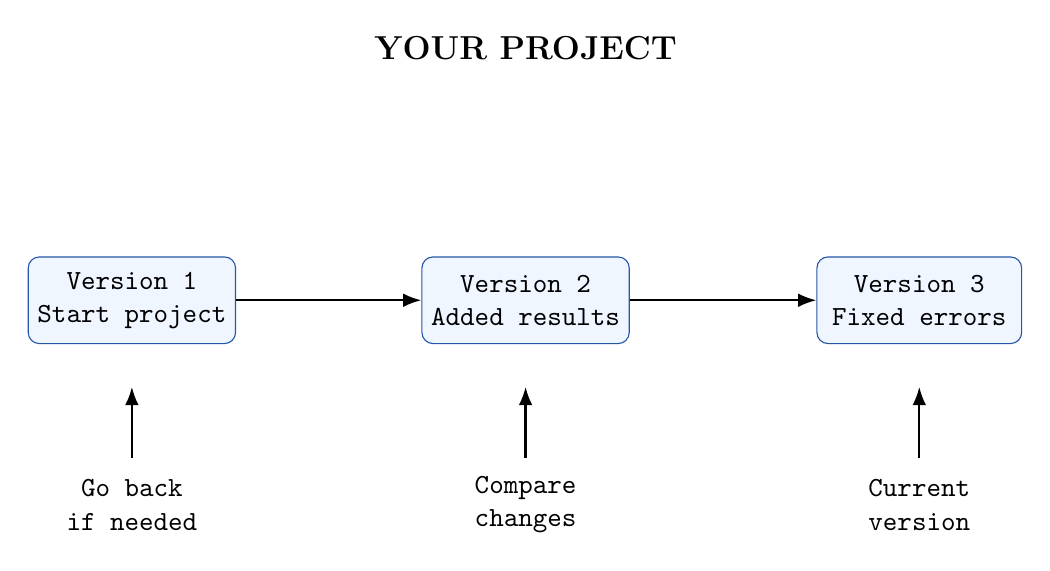
\begin{tikzpicture}[
    >=Latex,
    font=\ttfamily,
    version/.style={
        align=center,
        minimum width=2.6cm,
        minimum height=1.1cm
    },
    box/.style={
        rectangle,
        draw=black,
        rounded corners,
        draw=gitblue,
        fill=lightblue,
        minimum width=2.6cm,
        minimum height=1.1cm,
        align=center,
    }
]

% Project boxes
\node[box] (project1) at (0,-2) {Version 1 \\ Start project};
\node[box] (project2) at (5,-2) {Version 2 \\ Added results};
\node[box] (project3) at (10,-2) {Version 3\\ Fixed errors};

% Arrows between versions
\draw[->, thick] (project1.east) -- (project2.west);
\draw[->, thick] (project2.east) -- (project3.west);

% Up arrows
\draw[->, thick] (0,-4.0) -- (0,-3.1);
\draw[->, thick] (5,-4.0) -- (5,-3.1);
\draw[->, thick] (10,-4.0) -- (10,-3.1);

% Bottom labels
\node[align=center] at (0,-4.6) {Go back\\if needed};
\node[align=center] at (5,-4.6) {Compare\\changes};
\node[align=center] at (10,-4.6) {Current\\version};

% Title
\node[font=\normalfont\large\bfseries] at (5,1.2) {YOUR PROJECT};

\end{tikzpicture}
\end{center}

Each saved point is called a \textbf{commit}. For now, think of a commit as a saved version of your project.

For example:

\begin{code}
Commit 1 -> "Create project"
Commit 2 -> "Add introduction"
Commit 3 -> "Add results"
Commit 4 -> "Fix calculation"
\end{code}

Git remembers these versions for us. You don't need to remember every change yourself. You tell Git:

\begin{quote}
``Save this version.''
\end{quote}

Git remembers it.

Later, you can ask:

\begin{itemize}
    \item ``What did I change?''
    \item ``What versions do I have?''
    \item ``What was my project like before I made this change?''
\end{itemize}

That is why we can think of Git as a time machine for our project.

The bonus point is that Git works for many types of files, including programming/code files such as \texttt{.py}, \texttt{.c}, and \texttt{.cpp}, text files, documents, images, and more.

% =================================================
\section{Creating Our First Git Repository}
% =================================================

Now that we understand the problem, let's create our own Git time machine.

We will use a small project called \textbf{MyCalculator}.

% -------------------------------------------------
\subsection{Step 1: Create a Project Folder}
% -------------------------------------------------

Create a folder called:

\begin{code}
MyCalculator
\end{code}

Inside it, create a simple file:

\begin{code}
calculator.py
\end{code}

You can put 2--3 lines of simple Python code in the file, for example, a few \texttt{print()} statements.

Your folder should look like this:

\begin{code}
MyCalculator/
└── calculator.py
\end{code}

The folder contains our project. We want Git to keep track of what happens inside this folder.

% -------------------------------------------------
\subsection{Step 2: Tell Git to Track the Project}
% -------------------------------------------------

Open a terminal inside the \texttt{MyCalculator} folder and type:

\begin{code}
git init
\end{code}

You should see a message similar to:

\begin{code}
Initialized empty Git repository...
\end{code}

What just happened?

We told Git:

\begin{quote}
``Start keeping track of this project.''
\end{quote}

The folder is now a Git repository.

What is a repository?

A repository, or \textbf{repo}, is simply a project folder that Git is tracking.

\begin{center}
\textbf{Normal folder}
$\rightarrow$
\texttt{git init}
$\rightarrow$
\textbf{Git repository}
\end{center}

Git also creates a hidden \texttt{.git} folder inside the project. This is where Git stores the information it needs to maintain the project's history.

\textbf{Do not modify or delete the \texttt{.git} folder.}

% -------------------------------------------------
\subsection{Step 3: Ask Git What Is Happening}
% -------------------------------------------------

Now type:

\begin{code}
git status
\end{code}

Git will tell us about the current state of our project.

You may see something similar to:

\begin{code}
Untracked files:
    calculator.py
\end{code}

Git has noticed our file, but there is an important point:

Git knows the file exists, but we have not yet told Git to include it in a saved version.

This is what \textbf{untracked} means.

Think of it like this:

\begin{center}
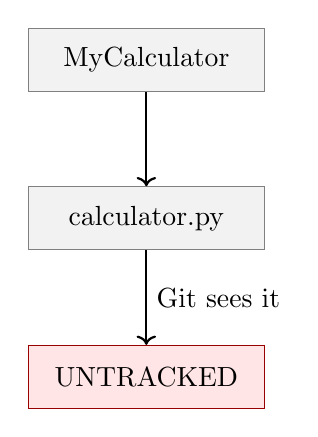
\begin{tikzpicture}[
    node distance=1.2cm,
    every node/.style={align=center},
    box/.style={
        rectangle,
        draw=gray,
        fill=gray!10,
        minimum width=3cm,
        minimum height=0.8cm
    }
]
\node[box] (folder) {MyCalculator};
\node[box, below=of folder] (file) {calculator.py};
\node[box, below=of file, fill=red!10, draw=red!60!black] (status) {UNTRACKED};

\draw[->, thick] (folder) -- (file);
\draw[->, thick] (file) -- node[right]{Git sees it} (status);
\end{tikzpicture}
\end{center}

We are now ready to make our first saved version.

% =================================================
\begin{checkpoint}{gitblue}
\textbf{Checkpoint 1 --- RA Approval: Repository Setup}

\textbf{Show your RA:}

\begin{itemize}
    \item The \texttt{MyCalculator} folder containing \texttt{calculator.py}.
    \item The repository initialized using \texttt{git init}.
    \item The output of \texttt{git status} showing \texttt{calculator.py} as an untracked file.
\end{itemize}

\textbf{RA Approval:} Confirm that the project has been correctly initialized as a Git repository and that the student understands the meaning of an untracked file.

\vspace{0.5em}

\textbf{Student Names:} \rule{5cm}{0.4pt} \textbf{RA Initials:} \rule{3cm}{0.4pt}
\end{checkpoint}

% =================================================
\section{A Quick Check}
% =================================================

At this point, remember these important terms:

\begin{center}
\begin{tabular}{>{\bfseries}p{3cm} p{9cm}}
\toprule
Term & Meaning\\
\midrule
Git & A tool that keeps the history of our project\\
Repository & A folder that Git is tracking\\
\texttt{git init} & A command that initializes a repository\\
\texttt{git status} & Shows the current state of our project\\
\bottomrule
\end{tabular}
\end{center}

Our first Git workflow:

\begin{center}
\textbf{Create project}
$\rightarrow$
\texttt{git init}
$\rightarrow$
\textbf{Git starts tracking the project}
$\rightarrow$
\texttt{git status}
$\rightarrow$
\textbf{See what Git knows about}
\end{center}

% =================================================
\section{Making Our First Commit: Saving a Version}
% =================================================

We have created our Git repository, and Git can see \texttt{calculator.py}. But there is a problem. Git knows that \texttt{calculator.py} exists, but we have not saved it as a version yet. Remember our time-machine idea?
We want to create our first save point:

\begin{center}
\textbf{Version 1}\\
``Create calculator''
\end{center}

To do this, we use two commands:

\begin{code}
git add calculator.py
git commit -m "Create calculator"
\end{code}

\textbf{Tip:} \texttt{git add -A} adds all the files in a folder instead of adding them one by one.

Let's understand them one at a time.

% -------------------------------------------------
\subsection{Step 1: Prepare the File with git add}
% -------------------------------------------------

Type:

\begin{code}
git add calculator.py
\end{code}

The \texttt{git add} command tells Git:

\begin{quote}
``I want to include this file in my next saved version.''
\end{quote}

Think of it like putting a document into a box before sealing the box.

\begin{center}
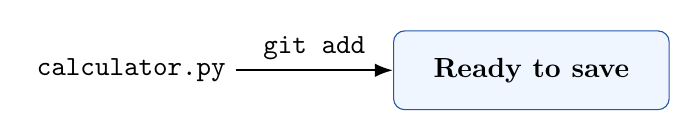
\begin{tikzpicture}[>=Latex]
\node (file) {\texttt{calculator.py}};
\node[draw=gitblue, fill=lightblue, rounded corners,
      minimum width=3.5cm, minimum height=1cm,
      right=2cm of file] (ready) {\textbf{Ready to save}};

\draw[->, thick] (file) -- node[above]{\texttt{git add}} (ready);
\end{tikzpicture}
\end{center}

You can check the situation with:

\begin{code}
git status
\end{code}

You should now see something similar to:

\begin{code}
Changes to be committed:
    new file: calculator.py
\end{code}

The important thing to notice is:

\begin{center}
\textbf{\texttt{git add} does not save a version.}
\end{center}

It prepares the changes that we want to save.

% -------------------------------------------------
\subsection{Step 2: Save the Version with git commit}
% -------------------------------------------------

Now type:

\begin{code}
git commit -m "Create calculator"
\end{code}

The \texttt{git commit} command tells Git:

\begin{quote}
``Save the prepared changes as a new version.''
\end{quote}

The \texttt{-m} allows us to give this version a message.

Our message is:

\begin{code}
"Create calculator"
\end{code}

So our first commit is:

\begin{center}
\textbf{Commit 1}\\
``Create calculator''
\end{center}

Think of the commit as pressing the \textbf{Save Point} button on our time machine.

\begin{center}
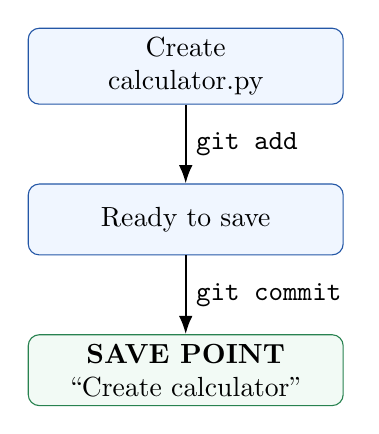
\begin{tikzpicture}[
    >=Latex,
    node distance=1cm,
    box/.style={
        rectangle,
        rounded corners,
        draw=gitblue,
        fill=lightblue,
        minimum width=4cm,
        minimum height=0.9cm,
        align=center
    }
]
\node[box] (project) {Create\\calculator.py};
\node[box, below=of project] (ready) {Ready to save};
\node[box, below=of ready, fill=lightgreen, draw=gitgreen] (save) {\textbf{SAVE POINT}\\``Create calculator''};

\draw[->, thick] (project) -- node[right]{\texttt{git add}} (ready);
\draw[->, thick] (ready) -- node[right]{\texttt{git commit}} (save);
\end{tikzpicture}
\end{center}

This saved point is called a \textbf{commit}.

% -------------------------------------------------
\subsection{Step 3: Check the Repository Again}
% -------------------------------------------------

Now run:

\begin{code}
git status
\end{code}

You should see something similar to:

\begin{code}
nothing to commit, working tree clean
\end{code}

This is good news!

It means there are no new changes waiting to be saved. Our project is now at a saved point.

% =================================================
\begin{checkpoint}{gitgreen}
\textbf{Checkpoint 2 --- RA Approval: First Commit}

\textbf{Show your RA:}

\begin{itemize}
    \item The \texttt{git add calculator.py} command.
    \item The \texttt{git commit -m "Create calculator"} command and its result.
    \item The output of \texttt{git status} showing a clean working tree.
\end{itemize}

\textbf{RA Approval:} Confirm that the student has successfully created the first commit and understands the difference between \texttt{git add} (prepare changes) and \texttt{git commit} (save a version).

\vspace{0.5em}

\textbf{Student Names:} \rule{5cm}{0.4pt} \textbf{RA Initials:} \rule{3cm}{0.4pt}
\end{checkpoint}

% =================================================
\section{Why Do We Need a Commit Message?}
% =================================================

Imagine that you make 20 commits but give every commit the message:

\begin{code}
Changes
\end{code}

After a few days, your history might look like:

\begin{code}
Changes
Changes
Changes
\end{code}

That isn't very helpful.

Instead, write a short message that explains what you changed:

\begin{code}
Create calculator
Add multiplication
Fix division
Add input validation
Improve error message
\end{code}

A good commit message should answer:

\begin{quote}
``What did I change in this version?''
\end{quote}

Keep it short and meaningful.

% =================================================
\section{The Important Difference: add vs commit}
% =================================================

Students often confuse these two commands, so remember:

\begin{center}
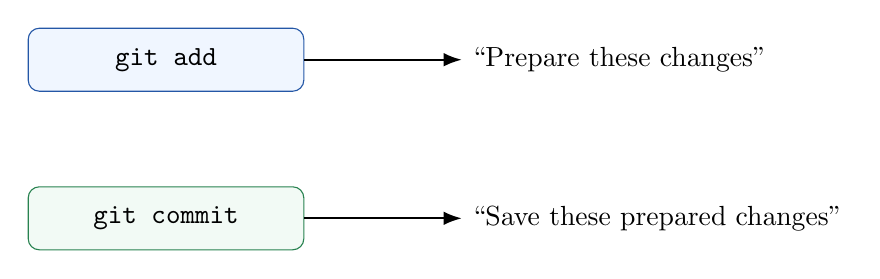
\begin{tikzpicture}[>=Latex]
\node[draw=gitblue, fill=lightblue, rounded corners,
      minimum width=3.5cm, minimum height=0.8cm] (add) {\texttt{git add}};
\node[right=2cm of add] (text1) {``Prepare these changes''};

\node[draw=gitgreen, fill=lightgreen, rounded corners,
      minimum width=3.5cm, minimum height=0.8cm,
      below=1.2cm of add] (commit) {\texttt{git commit}};
\node[right=2cm of commit] (text2) {``Save these prepared changes''};

\draw[->, thick] (add) -- (text1);
\draw[->, thick] (commit) -- (text2);
\end{tikzpicture}
\end{center}

Or, using our time-machine analogy:

\begin{center}
\begin{tabular}{ll}
\texttt{git add} & $\rightarrow$ Choose what goes into the save point\\
\texttt{git commit} & $\rightarrow$ Create the save point
\end{tabular}
\end{center}

So our basic workflow is now:

\begin{center}
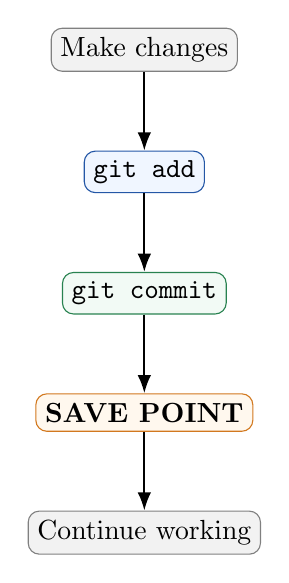
\begin{tikzpicture}[>=Latex, node distance=1cm]
\node[draw=gray, fill=gray!10, rounded corners] (make) {Make changes};
\node[draw=gitblue, fill=lightblue, rounded corners,
      below=of make] (add) {\texttt{git add}};
\node[draw=gitgreen, fill=lightgreen, rounded corners,
      below=of add] (commit) {\texttt{git commit}};
\node[draw=gitorange, fill=lightorange, rounded corners,
      below=of commit] (save) {\textbf{SAVE POINT}};
\node[draw=gray, fill=gray!10, rounded corners,
      below=of save] (continue) {Continue working};

\draw[->, thick] (make) -- (add);
\draw[->, thick] (add) -- (commit);
\draw[->, thick] (commit) -- (save);
\draw[->, thick] (save) -- (continue);
\end{tikzpicture}
\end{center}

% =================================================
\section{One Important Habit}
% =================================================

Commit when you have reached a meaningful point in your work.

For example:

\begin{code}
"Create calculator"
"Add multiplication"
"Add division"
"Fix input error"
\end{code}

You don't need to create a commit after every single character you type.

Think of a commit as:

\begin{quote}
``This is a useful version of my project that I may want to remember.''
\end{quote}

% =================================================
\section{Looking Back: Our Git History}
% =================================================

We have made our first commit.

But the real power of our time machine is that Git remembers our saved versions.

Let's see what Git remembers.

Type:

\begin{code}
git log
\end{code}

You should see something similar to:

\begin{code}
commit a82f31...
Author: Ali
Date:   ...

    Create calculator
\end{code}

This is our project's history.

Every time we make a commit, Git adds another entry to this history.

For example, after making a few more commits, our history might look like:

\begin{code}
commit c31a52...
    Add division

commit b72f10...
    Add multiplication

commit a82f31...
    Create calculator
\end{code}

Notice that the latest commit appears first.

Each commit also has a long-looking ID, such as:

\begin{code}
a82f31...
\end{code}

This is how Git identifies that particular commit.

For now, you don't need to understand how these IDs are created. Just remember:

\begin{center}
\textbf{Every commit has its own ID.}
\end{center}

The normal \texttt{git log} contains quite a lot of information.

For a quick look at our history, use:

\begin{code}
git log --oneline
\end{code}

You might see:

\begin{code}
c31a52 Add division
b72f10 Add multiplication
a82f31 Create calculator
\end{code}

This is often easier to read.

% =================================================
\section{What Did I Change?}
% =================================================

The history tells us which versions exist, but sometimes we want to know something more specific:

\begin{quote}
``What did I change after my last commit?''
\end{quote}

This is where \texttt{git diff} helps.

Let's try it.

First, open \texttt{calculator.py} and make a small change.

For example, imagine you had a print line in your file. Change:

\begin{code}
print("Hello")
\end{code}

to:

\begin{code}
print("Hello, Ali!")
\end{code}

\textbf{Do not commit the change yet.}

Now type:

\begin{code}
git diff
\end{code}

Git will show us the difference between our last saved version and our current file.

You may see something similar to:

\begin{code}
- print("Hello")
+ print("Hello, Ali!")
\end{code}

The symbols are simple:

\begin{itemize}
    \item \texttt{-} $\rightarrow$ something was removed or changed
    \item \texttt{+} $\rightarrow$ something was added or changed
\end{itemize}

So \texttt{git diff} answers:

\begin{quote}
``What have I changed since my last commit?''
\end{quote}

% =================================================
\section{The Complete Git Cycle}
% =================================================

We now know the basic commands needed to work with Git locally.

Imagine you are working on your calculator project.

You make some changes.

First, you can ask:

\begin{center}
\begin{tabular}{ll}
What is happening? & \texttt{git status}\\
What exactly did I change? & \texttt{git diff}\\
Prepare my changes & \texttt{git add .}\\
Save this as a new version & \texttt{git commit -m "Add multiplication"}\\
Show my saved versions & \texttt{git log --oneline}
\end{tabular}
\end{center}

The dot in \texttt{git add .} is part of the command.

Put together:

\begin{center}
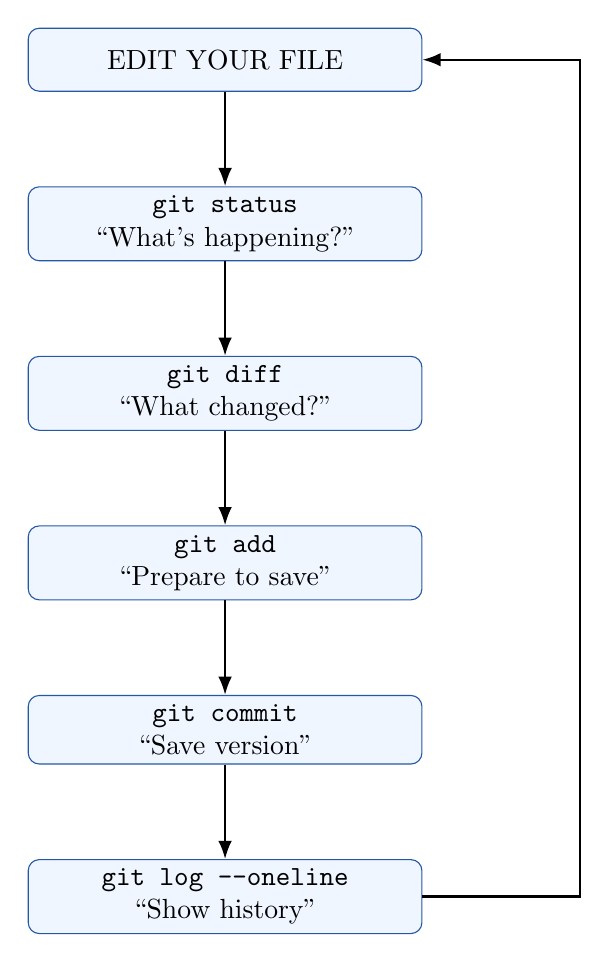
\begin{tikzpicture}[
    >=Latex,
    node distance=1.2cm,
    box/.style={
        rectangle,
        rounded corners,
        draw=gitblue,
        fill=lightblue,
        minimum width=5cm,
        minimum height=0.8cm,
        align=center
    }
]
\node[box] (edit) {EDIT YOUR FILE};
\node[box, below=of edit] (status) {\texttt{git status}\\``What's happening?''};
\node[box, below=of status] (diff) {\texttt{git diff}\\``What changed?''};
\node[box, below=of diff] (add) {\texttt{git add}\\``Prepare to save''};
\node[box, below=of add] (commit) {\texttt{git commit}\\``Save version''};
\node[box, below=of commit] (log) {\texttt{git log --oneline}\\``Show history''};

\draw[->, thick] (edit) -- (status);
\draw[->, thick] (status) -- (diff);
\draw[->, thick] (diff) -- (add);
\draw[->, thick] (add) -- (commit);
\draw[->, thick] (commit) -- (log);
\draw[->, thick] (log.east) -- ++(2,0) |- (edit.east);
\end{tikzpicture}
\end{center}

This is the basic Git workflow.

% =================================================
\begin{checkpoint}{gitorange}
\textbf{Checkpoint 3 --- RA Approval: Git History and Changes}

\textbf{Show your RA:}

\begin{itemize}
    \item The output of \texttt{git log --oneline} showing the project's commit history.
    \item At least three meaningful commits with descriptive commit messages.
    \item A modified \texttt{calculator.py} file.
    \item The output of \texttt{git diff} showing the changes that have not yet been committed.
\end{itemize}

\textbf{RA Approval:} Confirm that the student can view the project's history using \texttt{git log} and identify current uncommitted changes using \texttt{git diff}.

\vspace{0.5em}

\textbf{Student Names:} \rule{5cm}{0.4pt} \textbf{RA Initials:} \rule{3cm}{0.4pt}
\end{checkpoint}

% =================================================
\section{Your Git Time Machine}
% =================================================

After several commits, your project might have a history like this:

\begin{center}
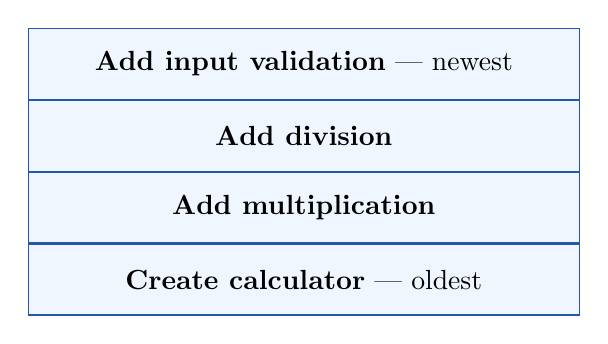
\begin{tikzpicture}
\node[
    draw=gitblue,
    fill=lightblue,
    minimum width=7cm,
    minimum height=0.9cm
] (v4) {\textbf{Add input validation} --- newest};

\node[
    draw=gitblue,
    fill=lightblue,
    minimum width=7cm,
    minimum height=0.9cm,
    below=0pt of v4
] (v3) {\textbf{Add division}};

\node[
    draw=gitblue,
    fill=lightblue,
    minimum width=7cm,
    minimum height=0.9cm,
    below=0pt of v3
] (v2) {\textbf{Add multiplication}};

\node[
    draw=gitblue,
    fill=lightblue,
    minimum width=7cm,
    minimum height=0.9cm,
    below=0pt of v2
] (v1) {\textbf{Create calculator} --- oldest};
\end{tikzpicture}
\end{center}

Each commit is a saved point in time.

Your current files are your work right now.

Your commits are the versions you have chosen to remember.

And \texttt{git diff} lets you see the changes between your current work and the last saved point.

That is the basic idea of Git:

\begin{center}
\Large
\textbf{Work}
$\rightarrow$
\textbf{See your changes}
$\rightarrow$
\textbf{Save a meaningful version}
$\rightarrow$
\textbf{Continue working}
\end{center}

You are building a history of your project as you work.

% =================================================
\section{Git Cheat Sheet}
% =================================================

\begin{center}
\begin{tabular}{>{\bfseries}p{6cm} p{6cm}}
\toprule
What do I want to do? & Command\\
\midrule
Start Git in my project & \texttt{git init}\\
See what is happening & \texttt{git status}\\
See what I changed & \texttt{git diff}\\
Prepare changes to save & \texttt{git add .}\\
Save a new version & \texttt{git commit -m "message"}\\
See my project history & \texttt{git log --oneline}\\
\bottomrule
\end{tabular}
\end{center}

% =================================================
\section{The Golden Rule}
% =================================================

Don't think of Git as a collection of commands to memorize.

Think of it as a conversation with your project:

\begin{center}
\begin{tabular}{ll}
``What is happening?'' & $\rightarrow$ \texttt{git status}\\
``What did I change?'' & $\rightarrow$ \texttt{git diff}\\
``Save this version.'' & $\rightarrow$ \texttt{git add + git commit}\\
``What have I saved?'' & $\rightarrow$ \texttt{git log}
\end{tabular}
\end{center}

And that is enough to get started with Git :-)

\end{document}
